\chapter{Triggers in Data Analysis}
  This appendix is written specifically for people who analyze the Hall-A experiments or other experiments with similar trigger settings in Hall-A. It could also be useful for people who are interested in the event distributions in the trigger system and the trigger efficiency.
  
  When a scattered electron goes through the detectors located in the detector hut of each High Resolution Spectrometers (HRS), the signals created in specific detectors are used to form different triggers. The traditional single-arm production trigger, T1 for HRS-R or T3 for HRS-L, requires both the S1 and S2m scintillator planes to fire within a narrow time window. During the E08-014, a gas Cerenkov detector (GC) was also added into the production trigger in order to exclude most of pions events, and to reduce the total event rate as well as the dead-time. The new production triggers were the coincidence of logic signals from S1, S2m and GC. The original triggers were still used for the PID study but were assigned with different names, T6 for HRS-R and T7 for HRS-L, respectively. 

 Besides the main production triggers, there are two other important triggers, T2 for HRS-R and T4 for HRS-L, designed for the study of trigger efficiencies. Both T2 and T4 require only one of S1 and S2m logic signals to be coincident with the logic signal from a third detector plane, such as the GC in this experiment. The T2 and T4 triggers are generated by sending logic signals from S1, S2m and Cerenkov into a programmable module,called MLU~\cite{halla_daq}.

 Ideally, before the pre-scaling, T6 (T7) should be exactly the same as T1 (T3),if the GC has 100\% detection efficiency and there are no background events. However, T6 (T7) had much higher event rates than T1 (T3) mainly because of the pion contamination. During the data taking, the rates of  T1 and T3  were kept as high as possible until the dead time became high. T3, T4, T6 and T7 were prescaled to fix their rates no more than 50 $\sim$ 100Hz. T5, the coincident trigger of T1 and T3, was not used in this experiment and its rate was set to zero. T8 was the signal from the CPU clock and was also maintained at very low rate. 
\begin{table}[htbp]
 \begin{tabular}{lcccccccc}
 \toprule
 Trigger:       &    T1   &   T2   &   T3   &   T4   &   T5   &   T6   &   T7   &   T8\\
 \midrule
 TDC Channel:   &     1   &    2   &    3   &    4   &    5   &    6   &    7   &    8\\
 Decimal:       &     2   &   $\mathrm{2^{2}}$   &    $\mathrm{2^{3}}$   &   $\mathrm{2^{4}}$   &   $\mathrm{2^{5}}$   &  $\mathrm{2^{6}}$  &   $\mathrm{2^{7}}$  &   $\mathrm{2^{8}}$\\
 Hex:           &    0x02 &   0x04 &   0x08 &   0x10 &  0x20  &  0x40  &  0x80  &  0x100\\
 \bottomrule
 \end{tabular}
% \centering
\caption{Triggers and their corresponding data types in data stream}
\label{trigger_table}
\end{table}

 All these trigger signals are sent to a 16-channel TDC port. Signals produced by an event can generate several types of triggers in a very narrow time window. Once one of the triggers is accepted by the DAQ system, all of the event's signals from detectors and other instruments are recorded by TDCs and ADCs. The trigger signals associated with this event are also stored. The analyzer decodes the TDC values of these triggers in Hex format and issues these values into a pointer-like variable in the \emph{\bf{T}} tree, "DBB.evtypebits". Table~\ref{trigger_table} lists the triggers and their corresponding values in different digital types.

 Based on this table, events belonging to the same trigger can be identified by applying cuts on the trigger variable. Note that an event can be affiliated with more than one trigger types. There are several kinds of trigger cuts used during data analysis, where differences are listed below:
 \begin{enumerate}
\item \textbf{DBB.evtypebits=0x02}: \\
    Selecting events which are associated with T1 trigger only. The cut returns a value of "1".
\item \textbf{(DBB.evtypebits\&0x02)==0x02}: \\
    Selecting events which are associated with T1 trigger and may also be associated with other triggers. The cut returns a value of "1".
\item \textbf{DBB.evtypebits$\gg1$\&1}: \\
    The same as (2).
\item \textbf{DBB.evtypebits \&(1$\gg$1)}: \\
    Exactly the same as (2) and (3), but returning a value of "2" instead of "1" (all non-zero values mean "TRUE")

\emph{The following two trigger cuts are not recommended:}
\item \textbf{DBB.evtype==1}: \\
     Selecting events only triggered by T1, and not by any other triggers coming within 5~ms window when the TS registers an event.This is almost the same as (1) except a slight difference caused by unknown reasons. 
\item \textbf{fEvtHdr.fEvtType==1}:\\
     Exactly the same as (5)
\end{enumerate}
\begin{figure}[!ht]
 \begin{center}
  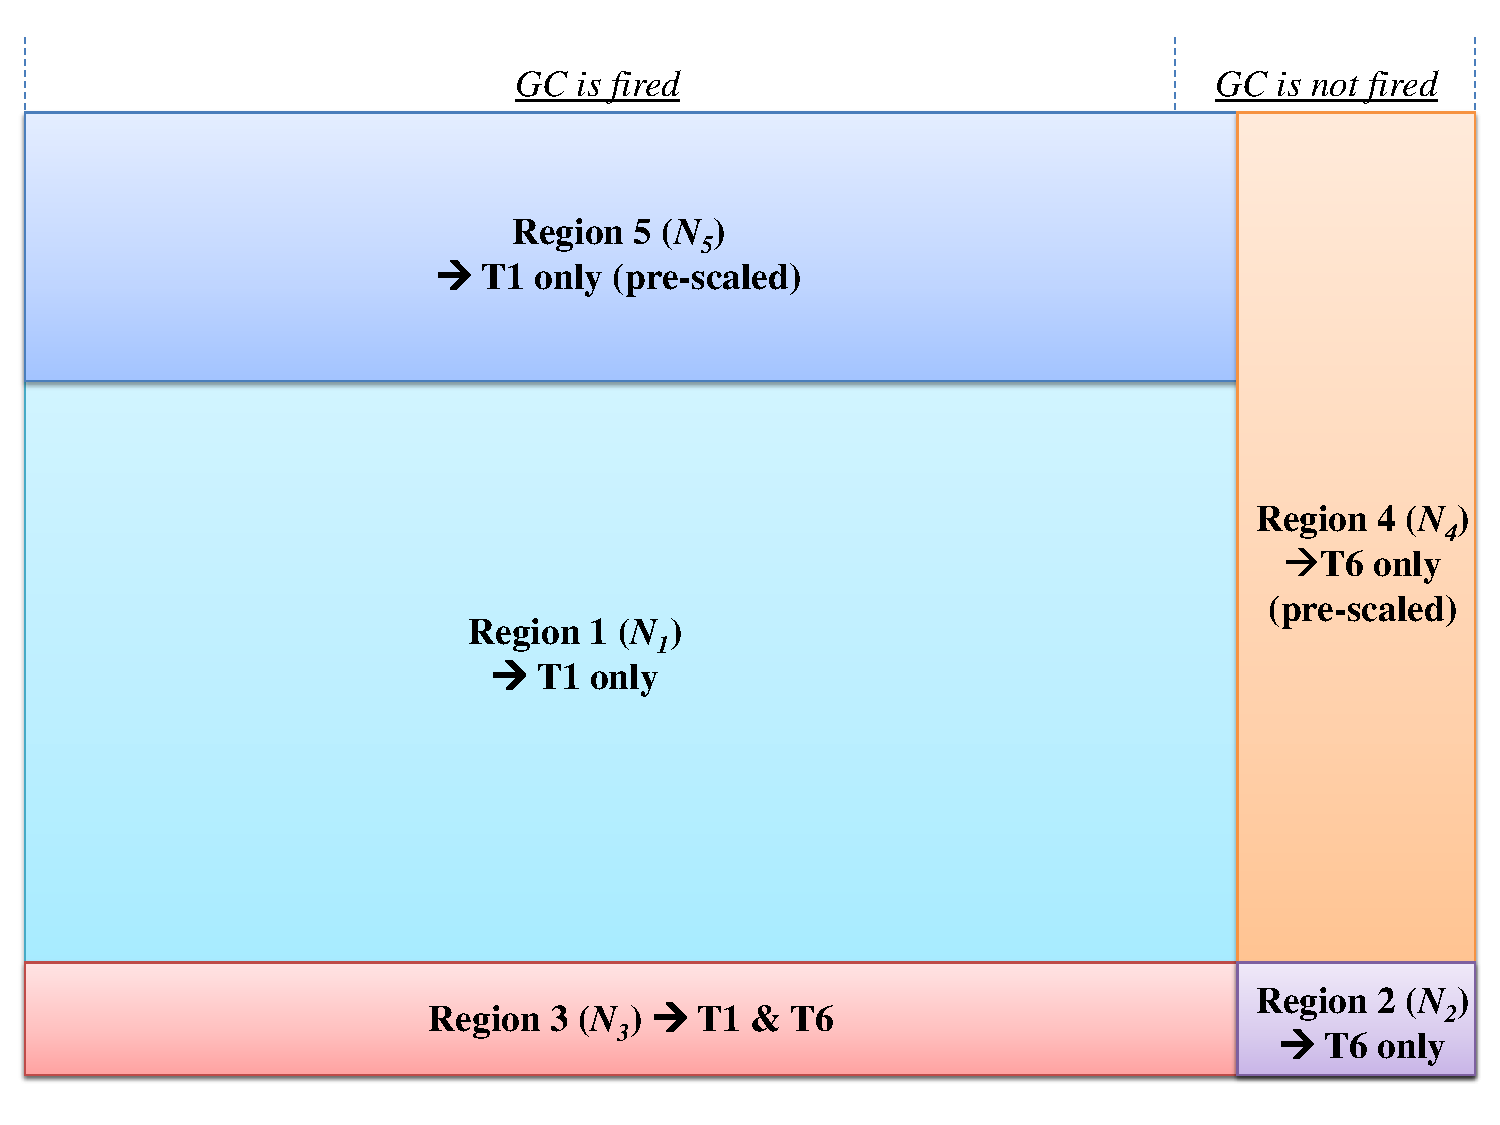
\includegraphics[width=0.6\textwidth]{./figures/trigger/trigger_region}
  \caption[A scheme of events with different trigger cuts]{A scheme of events with different trigger cuts. Each box denotes the number of events associated with certain trigger types. The size of each box does not necessarily reflect the real distribution of events in the data.}
  \label{trig_region}
 \end{center}
\end{figure}

  Not all the scattered electrons arriving in the detector hut can be recorded by the DAQ system because the detectors do not have 100\% detection efficiencies. Meanwhile, a certain portion of detected events are skipped as a result of pre-scaling. For each run, the pre-scale factors for different trigger types are recorded in the raw data as well as in the log files created at the start and at the end of each run. The total number of events from a trigger has to be corrected by the efficiency of the trigger system (i.e. the trigger efficiency) including the electronic, the computer and the detectors (S1, S2m and GC for E08014). The procedure to extract the trigger efficiency has been discussed in Section 5.5.1. In the rest of this section, all variables related to the number of events are assumed to have been corrected by the trigger efficiency.
   
  Assuming the total number of the scattered electrons which fire both S1 and S2m on HRS-R is given as the big box in Fig.~\ref{trig_region}, the area of each small box represents the number of electrons (events) associated with different trigger types after applying the pre-scale factors. Region 1 gives the number of events ($\mathrm{N_{1}}$) from T1 only, and region 2 gives the total number of event ($\mathrm{N_{2}}$) from T6 only. Region 3 represents the events associated with both T1 and T6 ($\mathrm{N_{3}}$). The portions of events which are not recorded due to the pre-scaling are given as $\mathrm{N_{4}}$ in Region 4 for T6 and $\mathrm{N_{5}}$ in Region 5 for T1, respectively. $\mathrm{N_{2}+ N_{4}}$ denotes the number of events which are not detected by the GC, and it should be small since the GC has a very high detection efficiency. So the relationship between the number of events in those regions and the pre-scale factors can given as:
 \begin{equation}
 PS1 = \frac{N_{1}+N_{3}+N_{5}}{N_{1}+N_{3}},  PS6 = \frac{N_{1}+N_{2}+N_{3}+N_{4}+N_{5}}{N_{2}+N_{3}}=\frac{N_{2}+N_{4}}{N_{2}},
\end{equation}
 where $\mathrm{N_{1}}$, $\mathrm{N_{2}}$ and $\mathrm{N_{3}}$ can be extracted from data by applying Trigger cuts as listed in Table~\ref{trigger_cut_table}.
\begin{table}[htbp]
 \begin{tabular}{lcc}
\toprule
 Events  &  Cut\\
\midrule
$N_{1}$  &  \textbf{DBB.evtypebits$\gg1\&1$\&\&!(DBB.evtypebits$\gg6\&1$)} \\
$N_{2}$  &  \textbf{DBB.evtypebits$\gg6\&1$\&\&!(DBB.evtypebits$\gg1\&1$)} \\
$N_{3}$  &  \textbf{DBB.evtypebits$\gg1\&1$\&\&DBB.evtypebits$\gg6\&1$}  \\
$N_{1}+N_{3}$  &  \textbf{DBB.evtypebits$\gg1\&1$}  \\
$N_{2}+N_{3}$  &  \textbf{DBB.evtypebits$\gg6\&1$}  \\
\bottomrule
  \end{tabular}
  \caption[Events types with different Trigger cuts]{Events types with different Trigger cuts}
  \label{trigger_cut_table}
\end{table}

 If the pre-scale factors are known, the total number of trigger events in the box can be mathematically calculated:
\begin{equation}
 N_{0} = N_{1}+N_{2}+N_{3}+N_{4}+N_{5}=PS6\times(N_{2}+N_{3}).
\end{equation}
However, since the pre-scale factor of T6 was set to be large enough to keep the trigger rate around 50Hz, the value of $N_{2}+N_{3}$ should be very small and the statistical error in $\mathrm{N_{0}}$ would be very large. However, $\mathrm{N_{1}}$ has much more statistics since T1 was maintained to have big trigger rate. Combined with $\mathrm{N_{4}}$ and $\mathrm{N_{5}}$, it gives the total number of electrons in that box as:
\begin{equation}
 N_{0} = N_{1}+N_{2}+N_{3}+N_{4}+N_{5}=PS1\times(N_{1}+N_{3})+PS6\times N_{2}.
\label{event0_1}
\end{equation}
where the term, $PS1\times(N_{1}+N_{3})$, denotes the number of events which fired the GC, while $PS6\times N_{2}$ is the number of electrons which did not fire the detector. 

\begin{figure}[!ht]
 \begin{center}
  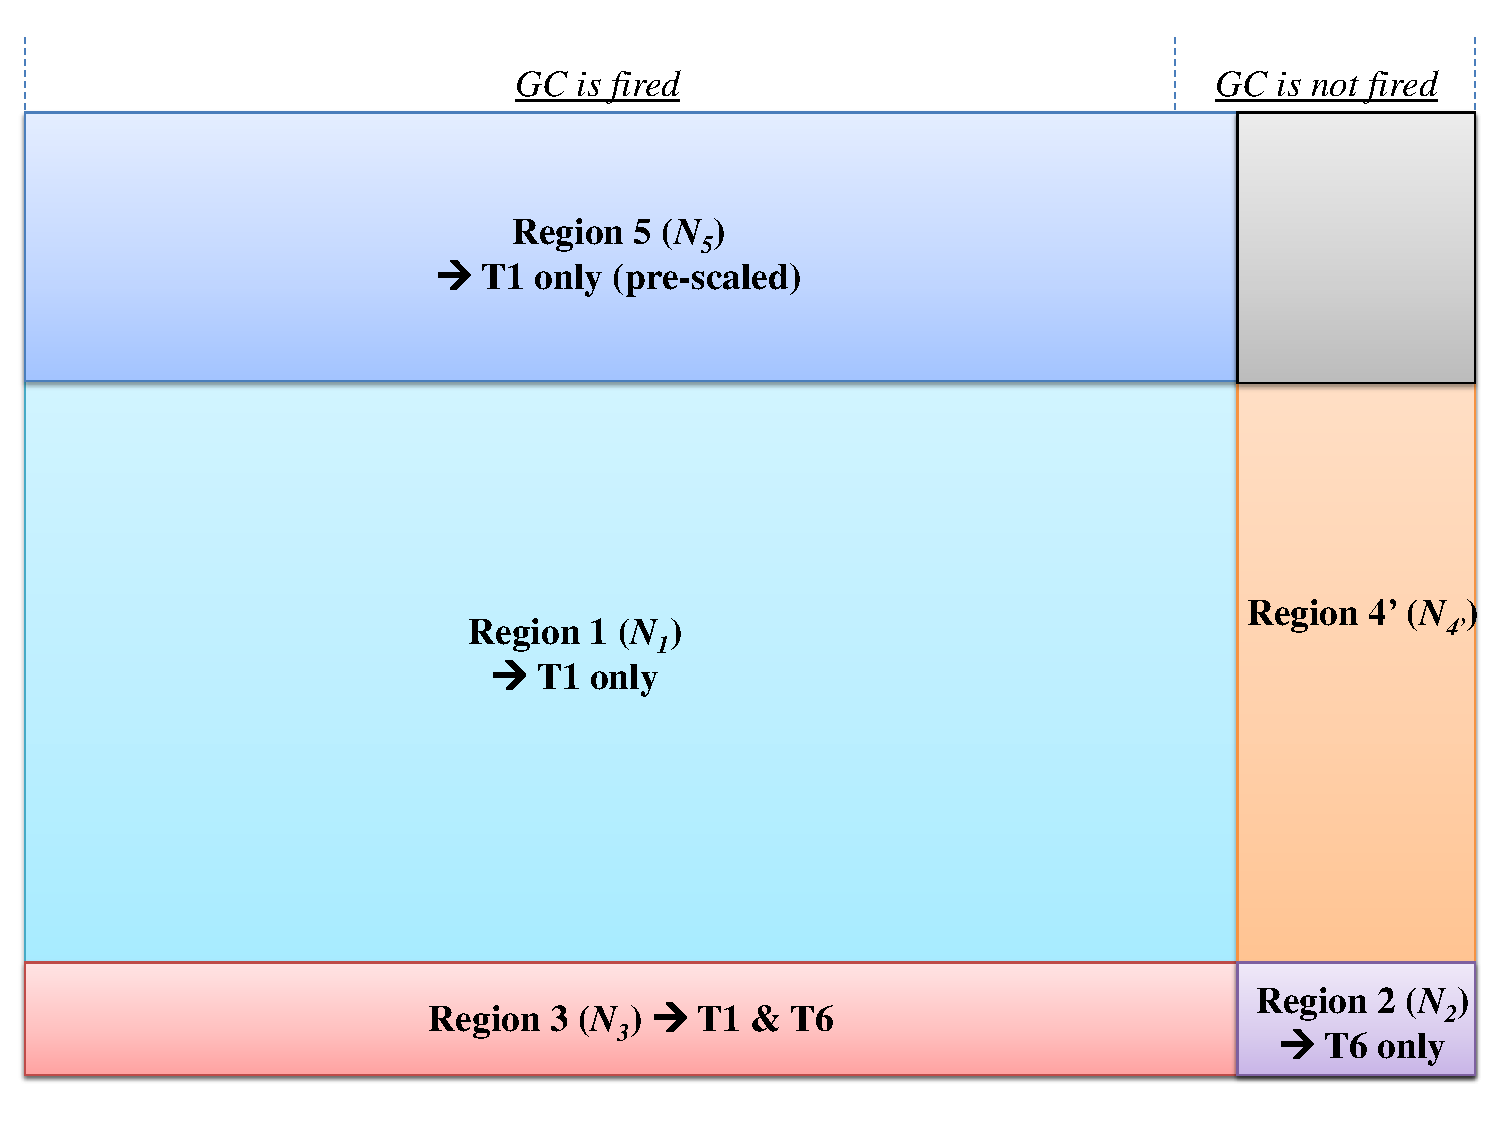
\includegraphics[width=0.6\textwidth]{./figures/trigger/trigger_region2}
  \caption[Another scheme of electrons with different trigger cuts]{Another scheme of electrons with different trigger cuts}
  \label{trig_region2}
 \end{center}
\end{figure}

Eq.~\ref{event0_1} can be further simplified. From Fig.~\ref{trig_region2}, a new region, called Region 4' ($N_{4'}$), can be defined:
\begin{equation}
\frac{N_{4'}}{N_{1}}=\frac{N_{2}}{N_{3}}=\frac{N_{2}+N_{4}}{N_{1}+N_{3}+N_{5}},
\end{equation}
which gives:
\begin{equation}
 N_{2}+N{4} = PS6\times N_{2} = PS1\times(N_{2}+N{4'}) = PS1\times(N_{2}+N_{1}N_{2}/N_{3}).
\end{equation}
and the relationship between PS1 and PS6 can be given by:
\begin{equation}
 PS6 = PS1(1+N_{1}/N_{3}).
\end{equation}

 So PS6 can be substituted by the formula above, and Eq.~\ref{event0_1} becomes:
\begin{equation}
 N_{0} = PS1\times(N_{1}+N_{3})\times \frac{N_{2}+N_{3}}{N_{3}}=\frac{PS1\times(N_{1}+N_{3})}{\epsilon},
\label{event0_2}
\end{equation}
where $\epsilon=\frac{N_{3}}{N_{2}+N_{3}}$ is the percentage of electrons firing GC when they pass through the detector, i.e. the exact definition of the GC detection efficiency. Since the number of events from T6 is very small, to reduce the statistical error, the typical way to get the detection efficiency of the GC is to select good electron samples from T1 events by applying a tight cut on the calorimeter and determining how many of them are detected by the GC (see Section 5.5.3): 
\begin{equation}
 \epsilon_{det}^{GC}=\frac{N^{GC}}{N^{Sample\_from\_Calo}}.
\end{equation}

 Based on the discussion above, $\mathrm{N_{0}}$ becomes straightforward: the total number of electrons passing through the HRS detectors is equal to the number of events triggered by S1, S2m and GC and corrected by the detection efficiency of the GC. It is important to emphasize that the value of $\mathrm{N_{0}}$ has to also be corrected by the trigger efficiency which is only related to the performance of S1 and S2m.
 
 The total number of trigger events from T3 on HRS-L can also be given in the same way.